% (c) Jakub Stejskal
% Master Thesis
% Performance Testing and Analysis of Qpid-Dispatch Router
% Chapter 5
\chapter{Implementation}
\label{Implementation}
This chapter describes the actual implementation details of components, described in the Chapter \ref{Analysis and Design}. The main part focuses on the Agent module and AMQP Inspector for MPT, which is implemented in Java and Groovy language. The other part describes the Topology Generator,\,---\,python package for automatic generation of dispatched topology based on user's metadata. Measurement data gathering and reporting done by MPT parts has already been mentioned in the Chapter \ref{Analysis and Design}.

\section{Topology Generation}
Qpid-dispatch has a lot of configurable attributes, which can influence the router behavior. These attributes can be set up with an AMQP management tool called \emph{qdmanage}\footnote{qdmanage\,---\,\url{https://qpid.apache.org/releases/qpid-dispatch-1.0.1/man/qdmanage.html}} or one can specify them directly in the configuration file. However, qdmanage needs human interaction, it is more comfortable to create configuration file for each specific test case. Hence, this initiates implementing automatic Topology Generator.

In case of network with multiple routers, it is uncomfortable to update configuration files for each router on a specific node. Topology Generator introduces an option to update only a single file with router specifications and leave generation and deployment to an automated script. The actual generation takes few simple steps to achieve correct configuration files. These steps are used in Ansible script and are described in the following.

\subsection{Configuration File Generation}
It is important to note that each configuration file is not generated by Topology Generator itself, but by Ansible playbook. Why do we need this approach? Since Qpid-dispatch is getting new versions every few months, they can change names of any configuration attribute or even erase them. This causes the problem, that when Qpid-dispatch is updated, then the code of Topology Generator has to be reviewed and updated too, otherwise one risks syntax errors in the configuration files. Such approach is not very stable, and hence the simple solution is to let Ansible do the final generation.

The trick is, that Ansible is able to fill-up any kind of passed \emph{Jinja2}\footnote{Jinja2\,---\,modern and designer-friendly templating language for Python \url{http://jinja.pocoo.org/docs/2.10/}} template only with data which are available. Basically, the Ansible playbook will get the configuration template and variables for router configuration files and creates proper configuration file. The script simply iterates through template and fills-up all available attributes. This process is repeated for every router machine in the Inventory file. Configuration variables are in JSON format, Ansible can recognize which variables are for particular machine.

\subsection{Template Generator}
Output configuration files are strictly based on input configuration template. This means that Ansible needs input template with specific attributes for each version. However, Qpid-dispatch offers a solution how to construct this template. Attributes are available inside a JSON file in the installation folder of Qpid-dispatch. To process this JSON file and create resulting configuration template we use a tool called \emph{qdrouter-jinja2}\footnotemark{}.

\footnotetext{qdrouter-jinja2\,---\,\url{https://github.com/rh-messaging-qe/qdrouter-jinja2}}

Qpid-dispatch configuration file is divided into the multiple section where each sections has its own attributes. For example there is a \emph{router} section with router name, mode, etc., and \emph{ssl} section with security attributes. Each section can be specified multiple times, but usually only the last one found is used. The exceptions are \emph{connectors}, \emph{listeners}, \emph{addresses} and \emph{link routes} that can specify multiple connection points and routing types on single router. In the Algorithm \ref{alg:ansible_template_generator} you can see pseudo-code of template generation process.

\begin{center}
	\begin{algorithm}[H]
		\LinesNumbered
		\DontPrintSemicolon

		\SetKwFor{forPy}{for}{:}{}
		\SetKwIF{If}{ElseIf}{Else}{if}{:}{else if}{else}{}
		\SetKw{in}{in}
		\SetKw{var}{var}

		\KwIn{\emph{attributes\_file}\,---\,input file in JSON format}
		\KwOut{output file in Jinja2 format}
		\var output = ''''\;
		\forPy{line \in attributes\_file}{
			\If{line.is\_attribute()}{
				output += line.attributeToJinja2()
			}
			\uElseIf{line.is\_section()}{
				output += line.sectionToJinja2()
			}
			\Else{
				output += line
			}
		}
		output.strip()\;
		\KwRet{output}
		\caption{Template generation by qdrouter-jinja2.}
		\label{alg:ansible_template_generator}
	\end{algorithm}
\end{center}

From the pseudo-code you can see that there are two kind of wrappers for processing the JSON. Their function is to make configuration sections and attributes optional and repeatable which is achieved by wrapping the sections and attributes with Jinja2 code. The attribute wrappers processes each attribute line into the following template snippet:

\begin{verbatim}
{%% if section.attribute is defined %%}
    attribute: {{ section.attribute }}
{%% endif %%}
\end{verbatim}

This code in template specifies, that if Ansible knows the variable \emph{section.attribute}, it will add a line with that attribute name and variable value into the configuration file. Key words section and attribute are just placeholders for real names such as \emph{connector} for section and \emph{host} for attribute. Output can then look like the following line:

\begin{verbatim}
		host: 10.0.0.1
\end{verbatim}

The section wrapper is more complex, because it has to wrap the start and the end of the section. This is handled by class methods \texttt{\textunderscore enter\textunderscore ()} and \texttt{\textunderscore exit\textunderscore ()} which allows you to implement objects that execute \texttt{\textunderscore enter\textunderscore ()} at start and \texttt{\textunderscore exit\textunderscore ()} at the end of some statement. Basically this class is created for each section and these methods are invoked before first and after last attribute. The \texttt{\textunderscore enter\textunderscore ()} method wraps start of each section with following code:

\begin{verbatim}
{%% if item.section_name is defined %%}
{%% for section_name in item.section_name %%}
section_name {
\end{verbatim}

The \textbf{\textunderscore exit\textunderscore ()} method closes the section with the following piece of code in the Jinja2 template:
\begin{verbatim}
}


\end{verbatim}

Since qdrouter-jinja2 parses JSON data from installed version of Qpid-dispatch on remote node it guarantees that the template will always correspond with specific router version. The template is saved in \emph{/tmp} folder on the remote machine where Ansible scripts can fetch it into the local folder and fill it up with data.

\subsection{Topology Generator}
Topology Generator is the main part of configuration generation and deployment. It process configuration variables for Ansible deployment scripts from the user specification. Topology Generator requires two parameters: the path to the Inventory and path to the graph file or topology type:

\begin{description}
	\item \textbf{Path to the Inventory}\,---\,Inventory is simple configuration file with list of nodes, connected to the network. Generator retrieves node names and types (router, broker) and use them during generation of variables. The generator creates specific sections and attributes based on node and graph types. Since broker configurations are not generated by this tool, it uses information only about specification of link routes to neighbours. Broker configuration is based on XML files, where user can specify Broker attributes. However, the future goal is to generate configuration for Broker too.
	\item \textbf{Path to Graph file}\,---\,Graph file is a simple YAML file which specifies node distribution in the network. It contains at least node name and links to another nodes. Beside the name, user can specify another node informations such as constructors, listeners, SSL profiles, etc. easily for each node. The whole file is loaded during initialization and is processed with the Topology Generator.
	\item \textbf{Topology Type}\,---\,Topology generator can create topology without graph file, but then it requires network type which will be generated. For example the topology type can be a line which puts all nodes into one line and generates connections between them.
\end{description}

Inner representation of network is realized by Python library \emph{NetworkX}\footnote{NetworkX\,---\,\url{https://networkx.github.io/documentation/latest/}}. It creates a graph as an object and offers manipulation with its attributes which are objects of nodes and links. Topology Generator is able to store information about network configurations as attributes of these objects. During the graph initialization, the generator stores basic information about nodes such as the name and the type from inventory or some additional information from the graph file. Basic algorithm of topology generation is depicted in the Algorithm \ref{alg:default_connections}.

However, the generation for each configuration section is more complex and is slightly different for sections for connections to another nodes. The generation is split into two parts based on the user's arguments: the first is generation of the default connections and the second is the generation of user specific sections from metadata file.

\begin{description}
	\item \textbf{Default Connections}\,---\,default connections corresponds to configuration for establishing connection between two devices in the network. To achieve this one has to configure listeners, connections, addresses and link routers (depending on second machine) on each router. This sections can be easily automatically generated only with the minimal knowledge about the network. The default connections are generated automatically when user specifies only hosts and topology type. The generator takes neighbours of each machine. Generator's output in that case is a file with variables for fully functional connections between machines. During the generation from the graph file each node has attribute which specifies if user wants the default connections. The Algorithm \ref{alg:default_connections} captures the default generation process.

	\item \textbf{User Specific Sections}\,---\,these sections are not needed for the proper communication inside the network. An example of this section can be SSL or auto-links settings. The generator loads data about these sections from graph file. Qpid-dispatch has a lot of setting, hence the generator does only the basic connectivity configuration without any specific settings if the user does not specify otherwise. You can see the user specific sections generation in the Algorithm \ref{alg:default_connections} as the part of the first \emph{for} statement. This generation part is done alongside with default connections generation.

\end{description}

Used algorithms are pretty straightforward. Since the generator is able to load IP addresses from inventory there has to be mechanism for automatic generation of proper port numbers for listeners and connectors. The problem is, that connectors of node X and listeners of directly connected node Y has to have same port numbers. It means, that node X connects to a specific port on node Y and node Y listens on that port. The initial port numbers is 5672, the default AMQP port, and it is incremented with each newly created listener. Hence, the listeners must be generated first on all nodes and then the connectors can be generated. This allows the access to port numbers of neighbor listeners via simple method and explains the double loop over nodes in the Algorithm \ref{alg:default_connections}.

\begin{center}
	\begin{algorithm}[H]
		\LinesNumbered
		\DontPrintSemicolon

		\SetKwFor{forPy}{for}{:}{}
		\SetKwIF{If}{ElseIf}{Else}{if}{:}{else if}{else}{}
		\SetKw{in}{in}
		\SetKw{var}{var}

		\KwIn{Inventory, Graph File/Topology Type}
		\KwOut{output file in JSON format}
		\var inventory = parse\_inventory(Inventory)\;
		\var graph = create\_graph(inventory, Graph File/Topology type)\;
		\var output = \{\}\;
		\forPy{node, neighbors \in graph.adjacency()}{
			output.update(generate\_listeners(node, neighbors))\;
			output.update(generate\_addresses(node, neighbors))\;
			output.update(generate\_specific(node, neighbors))\;
		}

		\forPy{node, neighbors \in graph.adjacency()}{
			connectors, link\_routes = generate\_connectors(node, neighbors)\;
			output.update(connectors)\;
			output.update(link\_routes)\;
		}
		\KwRet{output}
		 \caption{Default connectivity generation.}
		 \label{alg:default_connections}
	\end{algorithm}
\end{center}

\begin{center}
	\begin{algorithm}[H]
		\LinesNumbered
		\DontPrintSemicolon

		\SetKwFor{forPy}{for}{:}{}
		\SetKwIF{If}{ElseIf}{Else}{if}{:}{else if}{else}{}
		\SetKw{in}{in}
		\SetKw{var}{var}

		\KwIn{\emph{node}---node from graph, \emph{neighbors}}
		\KwOut{lists of connectors and link\_routes}
		\var connectors = []\;
		\var link\_routes = []\;
		\forPy{neighbor \in neighbors}{
			\If{neighbor.is\_router()}{
				connectors.append(connector\_setting)\;
			}
			\uElseIf{neighbor.is\_broker()}{
				connectors.append(connector\_setting)\;
				link\_routes.append(link\_route\_setting)\;
			}
		}
		\KwRet{connectors, link\_routes}
		 \caption{Connectors and link routes generation. The algorithm describes function \texttt{generate\_connectors()}.}
		 \label{alg:link_routes}
	\end{algorithm}
\end{center}

The Algorithm \ref{alg:link_routes} shows the generation process of connectors and link routers. The connectors are generated for each other network service (router/broker), but link routes are generated only in the case of the connection to the broker. The link route section then contains name or address of the connected broker, name of queue to which router will send the messages and specification of link route direction (input or output). For full-duplex connection to the broker one needs connector and two link routes from the router to the broker.

\subsection{Deployment}
At this point, everything is ready for creation the Ansible playbook to run all necessary tools and do the deployment of generated configuration files. Note, that each task can be executed on different machine based on the inventory.

The playbook combines all previously mentioned tools and also uses some features from Ansible role \emph{ansible-qpid-dispatch}\footnote{Ansible-qpid-dispatch\,---\,Ansible role for install
and setup Qpid-dispatch. The role is available at \url{https://github.com/rh-messaging-qe/ansible-qpid-dispatch}} such as start/stop handlers. These steps are added in any playbook or role, and can be used for automatic topology generation and deployment. The necessary things are Inventory and topology metadata for each test-case. In the following description you can see the list of deployment steps, that are executed on the control node (node where use the playbook):

\begin{description}
	\item \textbf{1. Install the Topology Generator}\,---\,Topology Generator is the main actor in the topology deployment so it is necessary to have it installed. Ansible takes care of it in the playbook.
	\item \textbf{2. Run the Topology Generator}\,---\,Topology Generator needs configuration files for proper execution. In play one just needs to specify the path to configuration files and Ansible will do all other things.
	\item \textbf{3. Include variables into Ansible}\,---\,this step loads the generated variables into memory. After this step, the script is ready to fill-up the template on remote machines.
\end{description}

Since Ansible offers smart system with variables inside the playbooks, one can assign all paths to configurations files to variable in the script or pass them with option during the playbook execution start. After these steps we are ready to execute few steps on the remote nodes:

\begin{description}
	\item \textbf{4. Install qdrouter-jinja2} and \textbf{generate templates}\,---\,this qdrouter-jinja2 is used to generate template. We need to install it on all of router nodes, because each router can have different version and it can affect the configuration file with deprecated attributes. After installation the templates are created.
	\item \textbf{5. Fill templates on remotes}\,---\,the script fills-up the template on each node. Since it has information about all nodes from configuration variables, it simply compares hostname with key from variables to assign proper data to each host.
	\item \textbf{6. Restart Qpid-dispatch}\,---\,after the change of configuration, we need to restart each machine and reload the configuration.
\end{description}

\section{Qpid-Dispatch Performance Module}
This section focuses on Maestro Agent implementation and updates of all other Messaging Performance Tool parts such as commands updates, extension of the Inspector and report changes. The Agent is implemented in Java and Groovy languages.

\subsection{MPT Preparations}
\label{MPT Preparations}
The first step during the development is to update the Maestro project structure by adding the new module called \emph{maestro-agent}. The agent is designed as the new independent service, which can be run after the building of the package by Maven. First, we need the main function for the agent, whoch is built with each new package. After the creation of main we have to create \emph{assembly.xml} which tells Maven which files has to be used for creation of new package during the build. The last step is to update all \emph{pom.xml} files, where are specified all dependencies and then, we are ready to build and start the implementation.

\subsection{Agent Module}
As it was mentioned in Subsection \ref{Extension Points}, the agent is an independent service running on the testing node. Since Maestro already has a similar services, we can reuse the already working parts. The Maestro has a class \texttt{MaestroWorkerManager} which represents a simple Maestro peer. This class has a several important methods which are inherited and used by Agent as well:

\begin{itemize}
	\setlength\itemsep{0em}
	\item \texttt{connect()}\,---\,this method connects each peer to the Maestro Broker. Based on the peer function, it also subscribes the peer to all needed topics. For example, the sender peer does not need subscription to agent commands topic. When this method throws an exception, the peer is not able to connect to Maestro Broker and the test fails.
	\item \texttt{noteArrived()}\,---\,this method catches incoming notes from Maestro Broker and invokes action based on the note.
	\item \texttt{handle()}\,---\,this method handles each received note. We overload this method to invoke specific handle method based on the received note type. Usually, the \texttt{handle()} methods in \texttt{MaestroWorkerManager} class only logs actions. For another functionality they are overridden in specific implementations of each peer.
\end{itemize}

Every action handle script is written in groovy, and so we needed a groovy script executioner. For this purpose, we created the class \texttt{GroovyHandler}. This class basically checks the handler file if it is executable and then tries to execute it. The handler file location is specified by the note payload. In that location one can specify more than one file; \texttt{GroovyHandler} checks and execute all of the files.

The main part of the Agent is the method called \texttt{callbacksWrapper()}. Since the Agent overrides \texttt{handle()} method to execute scripts from external point, every \texttt{handle()} method in the agent calls the \texttt{callbacksWrapper()}. The basic functionality is shown in the Algorithm~\ref{alg:agent_note_handle}. The reason why \texttt{sendReplyOk()} is sent everytime is that we need to know if thread was started. For example we can start the thread with the command execution 5 minutes after the start. We need the information if thread started successfully and then the information how the thread execution finished. However, the information about thread finish is sent by the handler itself. This is also reason why every external point handler creates its own thread. Naturally, the agent must serve other handlers during this time, and not wait 5 minutes for the finish of one of them and then handle the others.

\begin{center}
	\begin{algorithm}[H]
		\LinesNumbered
		\DontPrintSemicolon

		\SetKwFor{forPy}{for}{:}{}
		\SetKwIF{If}{ElseIf}{Else}{if}{:}{else if}{else}{}
		\SetKwIF{try}{catch}{catch}{try}{}{catch}{catch}{}
		\SetKw{in}{in}
		\SetKw{var}{var}

		\KwIn{externalPointPath, codeDir, note}
		\KwOut{sendReplyOk() or sendReplyFail()}

		\var thread = Thread()\;
		thread.start(groovyHandler.runExternalPoint())\;
		\etry{}{
			\var groovyHandler = GroovyHandler()\;
			groovyHandler.setInitialPath(externalPointPath)\;
			groovyHandler.setMaestroNote(note);
		}{
			sendReplyFail()\;
		}

		sendReplyOk()\;

		 \caption{Basic functionality of \texttt{callbacksWrapper()} method. \todo{Urcite vylepsit}}
		 \label{alg:agent_note_handle}
	\end{algorithm}
\end{center}

The other important method of Agent is the \texttt{handle()} override for \emph{AgentSourceRequest} note. After this note is received, the \texttt{handle()} method fetches a git repository URL from the note and tries to clone it. The current version offers to clone any public git repository and even the specific branch of the repository.

\subsubsection*{Agent Capabilities}
\label{Agent Capabilities}
The current implemented version of the Agent offers much more functions than was originally designed. The Agent does not focus only on Qpid-dispatch actions handling, but it can invoke action on node itself by executing extension points scripts. This makes agent usable also for Broker nodes, where it can simulate a real network behavior during the testing. The agent can also run 3rd party software on the node during the test, which can simulate any kind of  the unexpected behavior.

The agent is specific kind of Maestro Worker. This means, that agent connected to the Maestro Broker can publish messages during the test about its execution status or any additional information. You can see a simple communication with agent notes handling in the Figure \ref{fig:agent_demo}. The notes are send from front-end through Maestro Broker. Agent then invokes a specific handle method based on the received note. Inspector keeps inspecting the Qpid-dispatch by requests about his state every 15\,seconds.

\begin{figure}[H]
  \centering
  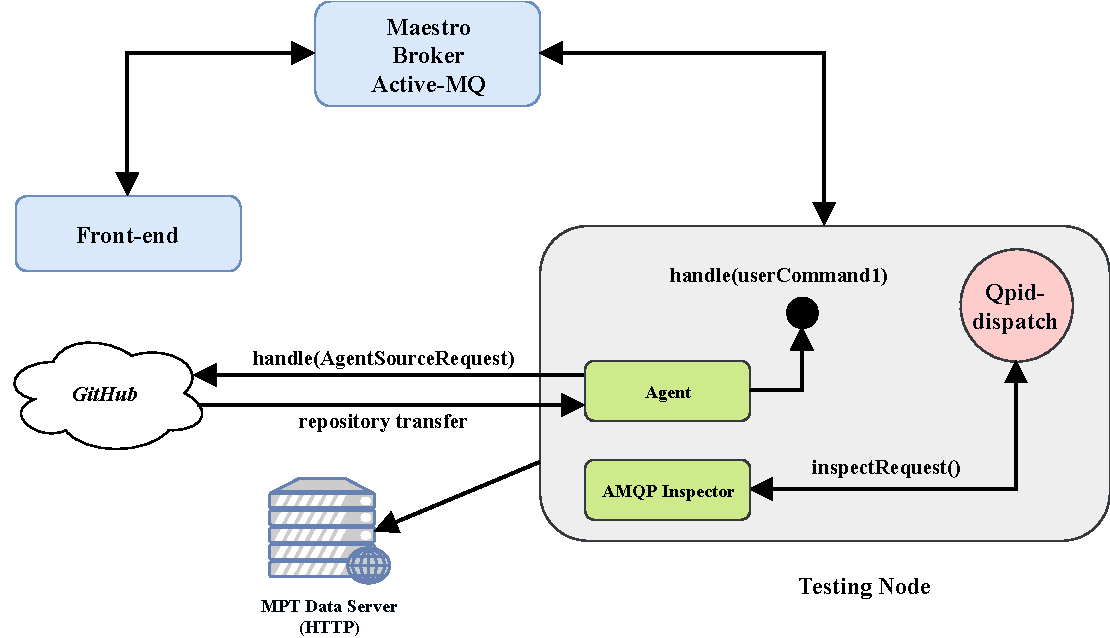
\includegraphics[width=13cm]{obrazky-figures/agent_demo.pdf}
  \caption{Communication inside the Maestro with agent notes handling.}
  \label{fig:agent_demo}
\end{figure}

\todo{dopsat neco?}

\subsection{AMQP Management Inspector}
\label{AMQP Management Inspector}
The collection of information about the router itself are not gathered by the agent. For this purpose, we developed a new type of Maestro Inspector specific for AMQP Management. AMQP Management is layered on top of the AMQP protocol and it access the inner data about the router by a simple requests and responses. Qdmanage tool has implemented operations for AMQP Management, however qdmanage is a Python tool and we want to integrate only Java code with AMQP Management requests into the Maestro. AMQP Management offers CRUD operations for router configuration and inter informations. For AMQP Inspector we are fine with only Read operation to get specific information about running the instance of Qpid-dispatch.



Using QPID JSM, update of maestro inspector start - start after the test start and pick up specific maestro inspector (artemis, ampq), update start inspector with payload.

 \todo{dopsat po implementaci}
